\documentclass{article}
\usepackage{graphicx} % Required for inserting images
\usepackage{geometry}
 \geometry{
 a4paper,
 left=25mm,
 right=25mm,
 top=30mm,
 bottom=30mm
 }

\usepackage[french]{babel}
\usepackage[T1]{fontenc}
\usepackage{lmodern}
\usepackage{hyperref}
\usepackage{wrapfig}

\title{Rapport de projet : Chat201 – édition thread \& réseau}
\author{Daniel DEFOING (\texttt{ddef0003}) \and 
        Belinda ÖZNUR (\texttt{bozn0003}) \and
        Haluk YILMAZ (\texttt{hyil0003})}
\date{\today}

\begin{document}
\pagenumbering{gobble}

\maketitle
\tableofcontents
\newpage

\pagenumbering{arabic}
\section{Introduction}
\noindent Ce rapport décrit globalement la conception du second projet dans le cadre du cours de Systèmes d'Exploitation
(INFO-F201). Il présente les choix de conception qui ont guidé notre développement, et les difficultés qui ont pu survenir durant celui-ci. Pour voir de façon précise les changements ayant eu lieu tout au long du projet et la contribution de chacun, veuillez consulter \hyperref[https://github.com/Daniel-Dfg/OS_Projet_2]{le repository GitHub de notre projet}.

\section{Choix du langage :pourquoi C++ plutôt que C ?}

\subsection*{Des outils qui facilitent le développement en général}
\noindent Une raison fondamentale qui a guidé cette décision est que C++ possède des fonctionnalités absentes en C tels que les références, les chaînes de caractères (ou \textit{strings}, qu'on a souvent subsitués aux \texttt{char*[]}) ou encore les classes. 

\noindent On peut aussi parler des conteneurs STL comme \texttt{std::vector} ou \texttt{std::queue} \cite{std::queue}, très utilisés dans cette implémentation du projet.


\noindent Or, dans le cadre du projet présenté ici, ces éléments apportent une pluvalue non négligeable en permettant de structurer un code de façon plus fine qu'en C ou de simplifier grandement certaines opérations. L'exemple le plus trivial qu'on peut donner de ceci est le passage de paramètres par référence plutôt que par pointeur dans certaines fonctions, qui permet une gestion plus sûre de la mémoire.

\subsection*{Des librairies qui fournissent des abstractions utiles pour ce projet}
\noindent On va illustrer ce point en parlant des \textit{threads}. En langage C, on utilisera \texttt{pthread.h} \cite{pthread.h} pour les gérer, alors qu'en C++ on a par exemple accès à la librarie standard \texttt{std::thread} \cite{std::thread}, qui permet d'abstraire certaines opérations de la librarie en C (par exemple, accéder au thread courant avec \texttt{std::this\_thread} \cite{std::thread}).

\noindent Utiliser C++ permet donc l'usage de certaines libraries standard absentes en C qui permettent d'abstraire des opérations de libraries \textit{correspondantes} en C.

\subsection*{Pas de perte notable à ne pas utiliser le langage C}
\noindent C++ reste évidemment compatible avec C : il n'existe pas d'opération en C infaisable exactement de la même façon en C++ \cite{StackOverflow-C}.
De plus, les deux langages étant connus pour leur rapidité d'exécution, la performance du C++ n'est pas dégradée de façon significative par rapport au C dans le cadre de ce projet.

\noindent L'utiliser permet donc de tirer parti ses abstractions discutées plus haut (voir 2 sections précédentes) tout en gardant une très bonne efficacité.


\noindent Tout ceci montre que les avantages majeurs ont été trouvés à utiliser C++ plutôt que C, alors qu’aucun avantage n’a été identifié en faveur de l’utilisation de C par rapport à C++. Ce choix du langage s’est donc naturellement imposé comme le plus adapté.

\section{Visualisation de l'architecture du programme}
\noindent Cette section discute des choix de conception du programme final, des considérations qui permettront au lecteur de mieux comprendre la nature de ces choix et des problèmes rencontrés qui en ont suivi.

\subsection{Le serveur en tant que \textit{point relais} des clients}
\noindent La structure d'un programme client-serveur tel que celui présenté ici peut être visualisée très simplement sous la forme d'un Graphe Étoile \cite{Graphe Étoile}, avec le serveur au centre et les clients aux extrémités de chaque branche. 
\begin{figure}[ht]
    \centering
    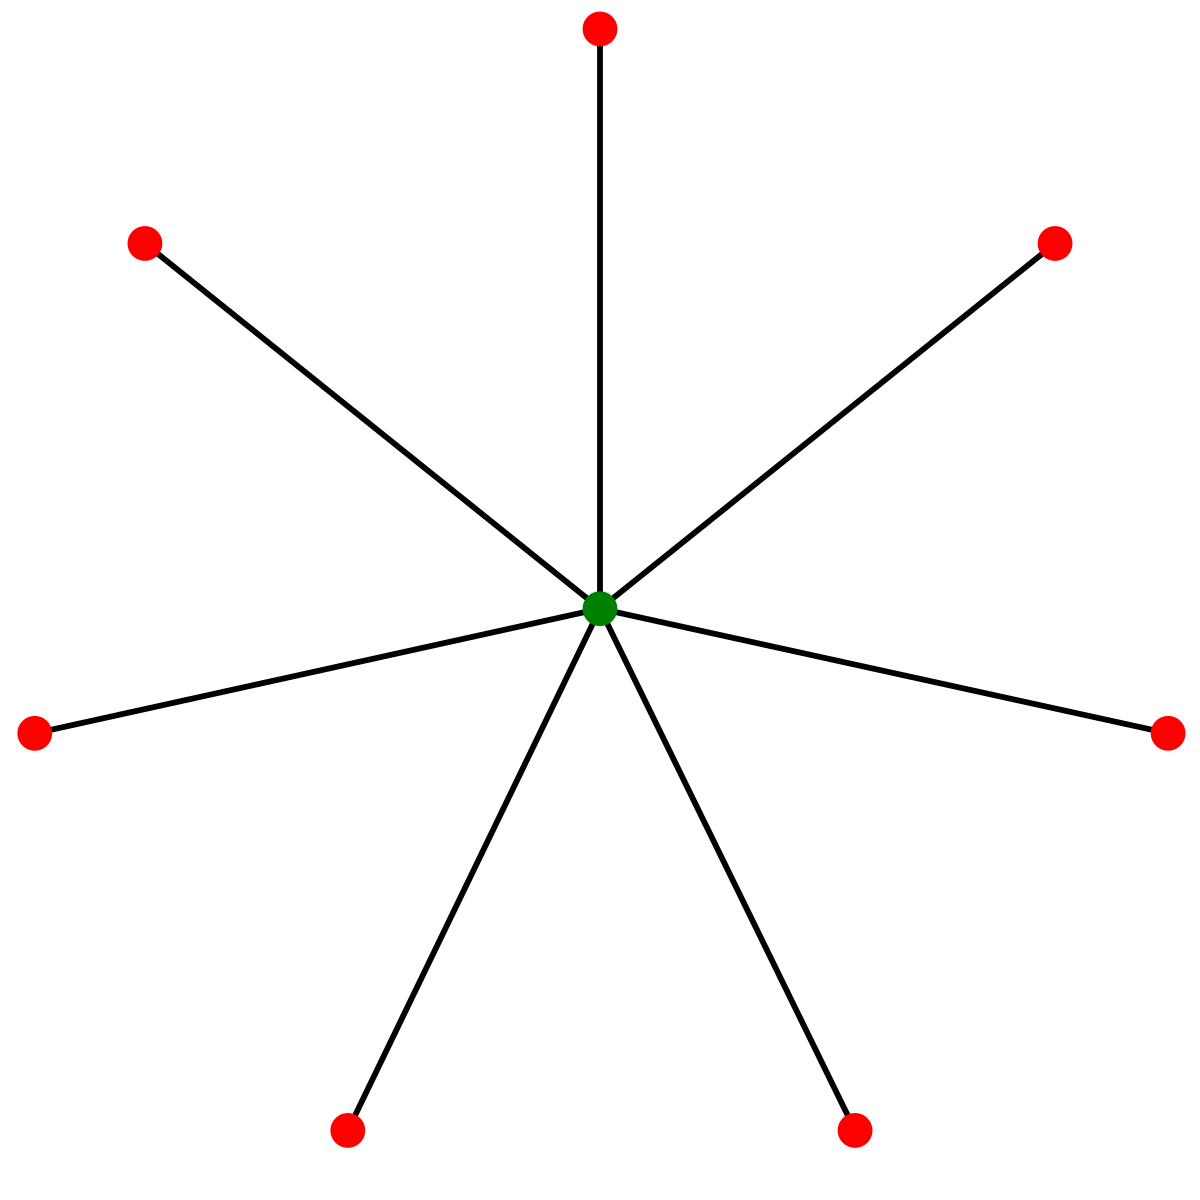
\includegraphics[width=0.25\linewidth]{etoile.png}
    \caption{\textit{Graphe Étoile typique.}}
\end{figure}

\noindent Cette représentation montre bien qu'un seul serveur se charge de \textit{relayer} les informations à passer d'un client à un autre ou d'un client vers lui-même (confirmation de (dé)connexion notamment). 

TODO : discuter du TCP/IP brièvement \cite{TCP-IP}

\noindent Dans la suite, on verra en profondeur la façon dont les sommets de ce graphe communiquent.

\subsection{Choix d'implémentation communs aux clients et au serveur}

\subsubsection{De la méthode d'envoi des messages}
\noindent Il a été décidé d'abstraire l'échange d'informations entre les clients et le serveur principalement par une classe \texttt{Message}. Un point très important qui découle de ce choix d'implémentation est qu'on a utilisé des \texttt{std::string} \cite{std::string} pour garantir une gestion dynamique de la mémoire et simplifier les opérations de manipulation des chaînes de caractère.

\subsection{Conception des clients}

\subsubsection{Deux FIFOs (ou \textit{files}) à vider en permanence}
\noindent Tout client possède deux \texttt{std::queue} \cite{std::queue} qu'il observe en permanence: une pour les messages qu'il envoie, et une pour ceux qu'il reçoit. 

\noindent Utiliser des \texttt{std::queue} n'ayant pas de taille limitée ainsi est une partie de la solution aux problèmes de synchronisation qui peuvent être rencontrés dans le cadre de ce projet. En effet, si un client reçoit plusieurs messages en même temps, les messages peuvent être \textit{push} à l'arrière de la FIFO servant et traités séquentiellement par le client qui la videra progressivement.


 \noindent Mais n'y a-t-il pas un risque que, si on envoie plusieurs messages simultanément à un même client, les deux messages risquent de corrompre la FIFO de réception du client (qui est un objet critique) en voulant s'insérer dedans en même temps ?


\noindent En principe, oui, c'est un problème qui peut survenir si on ne prend pas de précaution contre lui. C'est pour cela qu'on a fait usage de mutex (ou \textit{exclusions mutelles}) \cite{std::mutex} pour protéger la FIFO de réception côté client (éviter qu'elle reçoive plusieurs messages simultanément).


\subsubsection{Deux threads, deux FIFOs par client}
Ce point fait écho à la discussion de la section précédente sur l'usage de FIFOs côté client. 

\noindent Il faut préciser que le processus côté client se divise en deux \textit{threads}: un dédié à la réception des messages (qui doit donc vider et afficher le contenu de la FIFO de messages entrants) et un autre dédié à l'envoi de messages (qui doit donc en quelque sorte remplir la FIFO des messages à envoyer, puis la vider progressivement). 

\noindent Cette division du processus client en deux threads est due à des contraintes évidentes de performance et autorise le client à envoyer et recevoir des messages simultanément (gestion asynchrone des communications).

\subsubsection{Gestion de la (dé)connexion au serveur}
\noindent Tout client doit suivre le protocole TCP \cite{TCP-IP} pour initialiser sa connexion et doit s'identifier auprès du serveur.
(incomplet)


 Gestion de la déconnexion (quel thread tue l'autre, comment on se déconnecte) TODO :
 
1. Signal de terminaison envoyé aux deux threads

2. Attente de la fin des opérations en cours

3. Libération des ressources

4. Fermeture propre de la connexion

\subsection{Conception du serveur}

\subsubsection{De l'utilisation de \texttt{poll}}
\texttt{poll} \cite{poll} est l'outil qui a été choisi côté serveur pour gérer les connexions et envoi de messages par les clients. Il fonctionne ainsi \cite{poll} : 
\begin{enumerate}
    \item Initialiser un \texttt{std::vector} de \texttt{pollfd} (autrement dit, un vecteur de descripteurs de fichier pour pouvoir établir les communications). 
    \item Chaque client qui se connecte au serveur lui fait ajouter une nouvelle entrée au \texttt{std::vector}. Symétriquement, lors d'une déconnexion, il faut le parcourir pour supprimer l'entrée dans le vecteur du client qui s'est déconnecté.
    \item \texttt{poll} est \textit{edge-triggered}, ce qui signifie que le serveur est "notifié" en permanence quand des données sont disponibles. \cite{LevelEdgeTrigger} \cite{PollTrigger} Le serveur doit donc se charger de vider le vecteur de \texttt{pollfd} dès qu'il est notifié que des données à transmettre sont disponibles : en pratique, il \textit{boucle} sur le vecteur pendant toute sa durée de vie. 
    \item S'il observe que, dans un \texttt{pollfd}, il y a un message à transmettre, alors il recherche à qui le client envoyeur a voulu transmettre son message \footnote{En pratique, on recherche le nom du client récepteur dans un \texttt{std::unordered\_map} avec le nom du client comme clé et son \texttt{pollfd} comme valeur.} et, s'il existe, écrit dans le \texttt{pollfd} du client récepteur.


    Si le message à envoyer ne contient pas de nom de destinataire ou que le nom de destinataire spécifié ne fait référence à aucun client connecté, un message d'erreur est renvoyé. 
\end{enumerate}


\section{Améliorations non réalisées de l'implémentation actuelle}
\subsection{\texttt{epoll} comme alternative à \texttt{poll}}
\texttt{epoll} \cite{epoll} fonctionne de façon assez similaire à \texttt{poll}, mais a deux différences majeures:
\begin{enumerate}
    \item Il ne fonctionne que sur les systèmes d'exploitation Linux (ou basés sur Linux);
    \item Il peut être \textit{edge-triggered} (une "notification" est envoyée seulement lorsque des données sont disponibles) ou \textit{level-triggered} (une "notification" est envoyée tant que des données sont disponibles). \cite{LevelEdgeTrigger}
    \item On peut aller chercher les données uniquement des \textit{file desciptors} actifs (donc : ceux qui ont reçu un message) plutôt que de devoir itérer sur l'ensemble des \textit{file descriptors} disponibles (ce qui est malheureusement nécessaire pour \texttt{poll}). \cite{EpollTrigger}
\end{enumerate}

\noindent En clair, \texttt{epoll} est cité comme une alternative plus \textit{rapide} que \texttt{poll}, mais n'a pas été implémenté dans le cadre de ce projet car l'API est plus complexe à utiliser que celle de \texttt{poll}. Cela aurait tout à fait pu être fait en quelques jours supplémentaires cependant.

\subsection{Attente active pour les FIFOs côté client}
\noindent On l'a vu en section 3.3 (\ref{Conception des clients}), tout client est séparé en deux threads dont l'un gère une FIFO pour les messages entrants et l'autre les messages sortants. Cependant, l'implémentation actuelle de ce projet fait que le contenu des FIFOs est vérifié en permanence tant que le client est connecté \footnote{On pourrait en quelque sorte parler d'\textit{attente active} de la part du client. \cite{Attente Active} }

\noindent Par manque de temps, un système plus propre n'a pas pu être mis en place, mais on peut en esquisser le fonctionnement théorique (qui aurait certainement pu, comme pour \texttt{epoll}, être implémenté en quelques jours) :
\begin{enumerate}
    \item Initialement, la FIFO des messages entrants est vide. Dès qu'un message est envoyé au client, celui-ci commence à vider la FIFO. 
    \item Chaque nouveau message entrant correspond à une nouvelle "notification" pour le client, à une nouvelle tâche à faire : on peut donc facilement avoir un "compteur de tâches à faire" qui indique combien de fois le client doit extraire un message de la FIFO. Par exemple, si un client reçoit 3 messages en même temps, il est censé être notifié 3 fois et donc \texttt{pop()} le premier élément de la FIFO 3 fois (ce qui vide exactement la FIFO, en principe). 
    \item Lorsque la FIFO est vide, le client n'a pas besoin de vérifier son contenu en permanence.
\end{enumerate}

\section{Difficultés rencontrées et solutions trouvées}
\subsection{Problèmes de synchronisation}
\begin{itemize}
    \item côté serveur, accès concurrents (problème producteur-consommateur)
    \item Signaux asynchrones (mentionner la conception du SignalManager dans l'explication de la solution)
    \item ...
\end{itemize}

\subsection{Garantie de l'intégrité du contenu partagé par les clients}
\begin{itemize}
    \item Gestion des tailles limites (longueur de pseudos et de messages)
    \item Comment s'est-on assurés que le messages étaient bien transmis sans perte ?
\end{itemize}


\begin{thebibliography}{999}
    \bibitem{std::queue}
    \texttt{std::queue} - cppreference (dernière modification : 2024, 2 août)

    URL : \url{https://en.cppreference.com/w/cpp/container/queue}
    
    \bibitem{pthread.h}
        pthreads(7) — Linux manual page (dernière modification : 2024, 15 juin).

        URL : \url{https://www.man7.org/linux/man-pages/man7/pthreads.7.html}

    \bibitem{std::thread}
        \texttt{std::thread} - cppreference (dernière modification : 2023, 24 octobre).

        URL : \url{https://en.cppreference.com/w/cpp/thread/thread}

    \bibitem{StackOverflow-C}
        StackOverflow - \textit{Is there anything that can be done in C and not in C++ and the opposite way ? [closed]} (dernière modification : 2010, 9 décembre)
        
    URL : \url{https://stackoverflow.com/questions/4403328/is-there-anything-that-can-be-done-in-c-and-not-in-c-and-the-opposite-way}

	\bibitem{Graphe Étoile}
		Wikipedia : \textit{Graphe étoile} (dernière modification : 2019, 21 janvier)
        
        URL: \url{https://fr.wikipedia.org/wiki/Graphe_%C3%A9toile}

    \bibitem{TCP-IP}
    Wikipedia : \textit{Transmission Control Protocol} (dernière modification : 2024, 17 décembre)

    URL : \url{https://en.wikipedia.org/wiki/Transmission_Control_Protocol}

    \bibitem{std::string} 
    C++ Programming Language : \texttt{std::string} (dernière modification : inconnu)

    URL : \url{https://cpp-lang.net/docs/std/containers/strings/string/}

    \bibitem{std::mutex}
    \texttt{std::mutex} - cppreference (dernière modification : 2024, 6 mars)

    URL : \url{https://en.cppreference.com/w/cpp/thread/mutex}

    \bibitem{poll}
    poll(2) - Linux manual page (dernière modification : 2024, 15 juin).

    URL : \url{https://www.man7.org/linux/man-pages/man2/poll.2.html}


    \bibitem{LevelEdgeTrigger}
    StackOverflow - \textit{Level vs Edge Trigger Network Event Mechanisms} (dernière modification : 2022, 28 août).

    URL : \url{https://stackoverflow.com/questions/1966863/level-vs-edge-trigger-network-event-mechanisms}

    \bibitem{PollTrigger}
    StackOverflow - \textit{Is poll() an edge triggered function?} (dernière modification : 2013, 25 février).

    URL : \url{https://stackoverflow.com/questions/15072165/is-poll-an-edge-triggered-function?rq=3}

    \bibitem{epoll}
    epoll(7) — Linux manual page (dernière modification : 2024, 12 juin).

    URL : \url{https://www.man7.org/linux/man-pages/man7/epoll.7.html}

    \bibitem{EpollTrigger}
    StackOverflow - \textit{What is the purpose of epoll's edge triggered option?} (dernière modification : 2022, 25 septembre).

    URL : \url{https://stackoverflow.com/questions/9162712/what-is-the-purpose-of-epolls-edge-triggered-option?rq=3}

    \bibitem{Attente Active}
    Wikipedia : \textit{Busy Waiting} (dernière modification : 2024, 2 novembre).

    URL : \url{https://en.wikipedia.org/wiki/Busy_waiting}
\end{thebibliography}
Toutes sources consultées pour la dernière fois le 21/12/24, 16h.
    
\end{document}

